A construção de sistemas que sejam capazes de fornecer suporte ao
gestor em um processo de tomada de decisões tem sido um desafio ao
longo dos anos. A continuação será explicado a definição e arquitetura
de SAD, o SAD SustenAgro e os trabalhos relacionados.

\section{Definição de SAD}

Os Sistemas de Apoio à Decisão (SAD) são uma área de conhecimento
ampla e em continua evolução. A definição de SAD deriva da definição
de sistema, pois eles contêm um conjunto de partes organizadas para
um proposito comum, existem múltiplas definições do termo SAD, a continuação
serão apresentadas algumas definições que permitem explicar o proposito
deste tipo de sistemas.

\citet{Tweedale2016} define os SADs como sistemas software que visam
melhorar a tomada de decisão individual ou grupal, combinando o conhecimento
do(s) tomador(es) de decisão com dados relevantes de fontes confiáveis,
nos quais são aplicados métodos e modelos matemáticos para suportar
a análise, comparação e escolha de alternativas no processo de decisão.

\citet{heinzle2010semantica} define que os SADs apoiam o entendimento
de processos complexos, auxiliam na comparação dos fenômenos envolvidos
e suportam a análise e escolha de alternativas no processo de decisão.
Este entendimento do domínio surge da combinação das habilidades e
metodologias dos especialistas (humanos) à capacidade dos computadores
de acessar dados, estruturá-los em modelos, interpretar, formular
e avaliar alternativas e cenários distintos.

O conhecimento dos especialistas do domínio está implícito nos SADs.
\citet{Evans:2003:DDT:861502} explica que existe uma necessidade
de modelar o conhecimento chave de um domínio em um modelo, para permitir
a comunicação e colaboração entre especialistas de domínio e os desenvolvedores,
pelo qual o modelo de conhecimento dos especialistas será objeto da
pesquisa. O processo de modelagem pode ser lento e custoso, já que
os dois grupos de profissionais têm \foreignlanguage{english}{\emph{Backgrounds}}
diferentes, que dificultaram o processo de desenvolvimento e testes
de um SAD.

Os especialistas de domínio e os desenvolvedores, pelo geral são de
organizações diferentes, o que dificulta ainda mais o processo, pelo
qual foram pesquisados modelos que facilitem o entendimento entre
os dois tipos de profissionais e desenvolvida uma pesquisa ao redor
deste tópico.

A continuação será apresentada a arquitetura dos SAD e a importância
dos modelos de conhecimento existentes dentro um SAD. 

\section{Arquitetura para Sistemas de Apoio à Decisão}

A arquitetura de um software define a organização dele em termos de
componentes, de interconexões, e das interações com sistemas externos
\citep{de1997software}. A arquitetura fornece as informações de como
os componentes dela se relacionam, explicando a parte externa das
ligações entre seus elementos, sendo que as implementações internas
não são consideradas parte da arquitetura \citep{sei2006architecture}.

Estas partes são descritas por meio da arquitetura representada na
figura \ref{fig:Componentes-SAD}, representando o processo realizado
pelos SADs, no qual recebem uma entrada, fazem o processamento dela
e retorna resultados que são analisadas pelo tomador(es) de decisão
a través da tecnologia computacional \citep{Tweedale2016}. 

\begin{figure}[H]
\noindent \begin{centering}
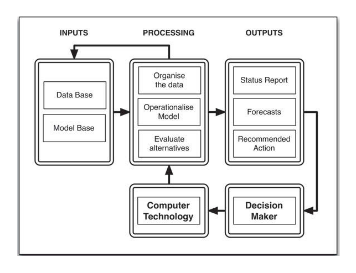
\includegraphics[width=0.8\columnwidth]{figures/DSS}
\par\end{centering}
\caption{Componentes de um SAD.\label{fig:Componentes-SAD} }

\fadaptada{Tweedale2016}
\end{figure}

A Figura \ref{fig:Componentes-SAD} mostra os componentes de um SAD,
que são: 
\begin{description}
\item [{I\foreignlanguage{english}{nputs}}] corresponde às entradas do
sistema, composta dos dados que serão processados e dos modelos de
conhecimento dos especialistas. Os dados estão armazenados em bancos
de dados e os modelos pelo geral estão implícitos no SAD ou podem
estar em uma base de conhecimento. Esses dois componentes devem ser
o mais precisos e completos possíveis para garantir respostas confiáveis
do sistema.
\selectlanguage{english}%
\item [{Processing}] \foreignlanguage{brazil}{está composto pelos modelos
e métodos de organização e processamento dos dados, que tem restrições
para avaliar as alternativas de resposta. Os métodos podem ser de
tipo matemáticos, que processam os dados e geram os resultados do
sistema.}
\item [{Outputs}] \foreignlanguage{brazil}{são os resultados do processamento
dos inputs e permitem comparar as alternativas de decisão. As saídas
comuns são relatórios, previsões e recomendações, que são apresentados
por meio de uma interface de usuário para facilitar o entendimento
e interação por parte dos usuários.}
\end{description}
Durante a evolução dos SAD, várias melhorias aconteceram, entre elas
o desenvolvimento da Web permitiu integrar novas técnicas no processamento
dos dados, tecnologias na representação visual de resultados e no
uso colaborativo por parte dos usuários \citep{Shim2002}. Também
existe a tendência da integração com métodos de inteligência artificial,
para estender a aplicabilidade dos SAD a problemas complexos. 

Uma variação dos SADs integra bases de conhecimento que suportam inferência,
permitindo o desenvolvimento de \foreignlanguage{english}{Expert Systems}
e \foreignlanguage{english}{Knowledge Based Systems.} Esses sistemas
são classificados como \foreignlanguage{english}{Rule Based Systems}
\citep{Tweedale2016}, os quais estabelecem o escopo desta pesquisa. 

Um tipo de SAD que usa bases de conhecimento, são os que usam ontologias
para representar o conhecimento dos especialistas, permitindo definir,
classificar, relacionar e inferir conhecimento. 

A continuação será apresentado o SAD SustenAgro baseado em conhecimento,
que suporta a avaliação da sustentabilidade em cana-de-açúcar a través
do uso de ontologias.

\section{SAD SustenAgro\label{sec:SAD-SustenAgro}}

Um domínio de conhecimento caracterizado pela sua complexidade são
os sistemas produtivos agrícolas. Eles envolvem fenômenos de natureza
diversa \citep{simon1991architecture}, integrando aspectos ambientais,
sociais e econômicos.

Particularmente, o setor produtivo produtivo da cana-de-açúcar é extremamente
importante para a economia do estado de São Paulo e do Brasil, devido
ao fato de ser uma das principais culturas produzidas no país \citep{Storquato2015}.
Atualmente a cana-de-açúcar é a mais importante fonte de energia renovável
no Brasil \citep{seabra2011life}, permitindo a produção de etanol
e energia eléctrica, além de ter mais de 20 subprodutos, entre eles
açúcar, etanol, bioeletricidade, bioplásticos e Hidrocarbonetos \footnote{\url{http://sugarcane.org/sugarcane-products}}. 

A produção da cana-de-açúcar e dos subprodutos dela, influem em aspectos
ambientais consumindo recursos naturais, em aspectos sociais envolvendo
pessoas na produção e em aspectos econômicos na comercialização. Esses
aspectos fazem complexo manter a produtividade atualmente e no futuro.
Por essas razões, a Embrapa Meio Ambiente escolheu especificamente
o sistema produtivo da cultura de cana-de-açúcar na região centro-sul
do Brasil, como sistema piloto para desenvolver métodos e software
de avaliação da sustentabilidade (apêndice \ref{chap:Sustainability_Assessment}).

Dada a complexidade da análise da sustentabilidade em sistemas de
produção agrícola, os pesquisadores da Embrapa Meio Ambiente trabalharam
na definição de métodos que permitissem avaliar a sustentabilidade
de maneira integral \citep{Singh2012281}. Por essa razão, desenvolveram
um método que aborda a avaliação em termos de indicadores, simplificando
a complexidade deste sistema agrícola. Cada indicador mede um determinado
aspecto crítico no sistema produtivo, para determinar o quão sustentável
ele é. A partir da análise de cada indicador, é possível gerar recomendações
de medidas corretivas para as unidades produtivas ou para o embasamento
de políticas públicas que incentivem a sustentabilidade. A definição
conceitual do processo de avaliação está detalhada no apêndice \ref{chap:Sustainability_Assessment}. 

A partir do método de avaliação SustenAgro, foi desenvolvida uma ferramenta
de avaliação da sustentabilidade intitulada SAD SustenAgro que implementa
o método SustenAgro por meio de um sistema de apoio a decisão e que
consegue adaptar-se às mudanças do domínio.

O SAD SustenAgro suporta a avaliação da sustentabilidade em cana-de-açúcar
no centro-sul do Brasil. A figura \ref{fig:SustenAgro-arquitetura-inicial}
apresenta a arquitetura inicial do SAD SustenAgro, a qual corresponde
a um sistema de informação tradicional, que requer a intervenção de
desenvolvedores de software, para definir ou atualizar o conhecimento
dos especialistas implícito no SAD.

\begin{figure}[h]
\begin{centering}
\includegraphics[width=0.6\columnwidth]{\string"figures/SustenAgro Initial Architecture\string".eps}
\par\end{centering}
\caption{SustenAgro arquitetura inicial.\label{fig:SustenAgro-arquitetura-inicial}}
\end{figure}

Os especialistas em sustentabilidade definiram o SAD Sustenagro com
as seguintes características:
\begin{itemize}
\item Sistema web com banco de dados para armazenar e recuperar as informações
do sistema.
\item Integração e implementação do método SustenAgro de avaliação de sustentabilidade,
descrito no apêndice \ref{chap:Sustainability_Assessment} 
\item Flexibilidade para adaptar o método SustenAgro a outras culturas.
\item Integração com sistemas de georreferenciamento.
\item Desenvolvimento de \foreignlanguage{english}{widgets} especificas
\footnote{\selectlanguage{english}%
Widgets\foreignlanguage{brazil}{ refere-se à componentes visuais dos
sistemas web }\selectlanguage{brazil}%
} para mostrar resultados obtidos: \foreignlanguage{english}{Sustainability
Matrix }e \foreignlanguage{english}{Sustainability Semaphore,} explicadas
no capítulo \foreignlanguage{english}{\ref{chap:SustenAgro}}
\item Geração de relatórios e de recomendações de sustentabilidade.
\end{itemize}
Um dos problemas identificados foi que os especialistas não tinham
uma definição clara do SAD SustenAgro. Pelo que foi necessário realizar
um levantamento de requisitos, descrito no capítulo \ref{chap:SustenAgro},
para definir os requisitos funcionais (essenciais) e não funcionais
(desejáveis). Além disso, foi necessário reestruturar o desenvolvimento
do SAD SustenAgro para que fizesse parte do processo de pesquisa.

O SAD SustenAgro faz parte de um conjunto de ferramentas de avaliação
definidas pela Embrapa Meio Ambiente. A partir do analise das ferramentas
similares ao SAD SustenAgro, foi evidenciada a necessidade de fornecer
métodos e ferramentas computacionais que organizem a informação. Para
apoiar aos especialistas a tomar decisões baseadas em conhecimento,
permitindo simplificar a resolução de problemas que de outra maneira
não seriam triviais. 

Exatamente foi identificado que ditos sistemas tinham em comum um
método de avaliação que processava de maneira matemática um conjunto
de dados e gerava relatórios com resultados da avaliação, gráficos
e recomendações. As ferramentas analisadas foram:
\begin{enumerate}
\item Sistema Innova-Tec: avaliação do impacto da inovação tecnológica\footnote{\url{http://www.cnpma.embrapa.br/forms/inova_tec.php3}}.
\item Sistema Nano-Tec: avaliação do impacto das nanotecnologias\footnote{\url{https://www.embrapa.br/en/busca-de-publicacoes/-/publicacao/951543/metodologia-para-avaliacao-de-impactos-das-nanotecnologias-metodo-e-software-impactos-nanotec} }.
\item Sistema GMP-RAM v.1.1: avaliação de Risco de Plantas Geneticamente
Modificadas (GMP \nomenclature{GMP}{Genetically Modified Plants})\footnote{\url{http://www.cnpma.embrapa.br/forms/gmp_ram.php3}}
\item Software para avaliação de segurança e impactos de plantas geneticamente
modificadas\footnote{\url{http://www.cnpma.embrapa.br/nova/mostra2.php3?id=857}}
\item Sistema Atlantis: Sistema para levantamento e sistematização da informação
técnica em temas de pesquisa, tecnologias e inovação. \footnote{\url{https://www.embrapa.br/en/busca-de-produtos-processos-e-servicos/-/produto-servico/2102/atlantis---atlantis}}
\end{enumerate}
Uma característica importante em ditos sistemas foi a existência de
conceitos de domínio especifico na organização dos dados de entrada
dos SAD e no método de avaliação. Esta característica permite identificar
que cada um dos sistemas requiriu um processo de modelagem dos conceitos
do domínio por parte dos desenvolvedores. 

Principalmente identificou-se que a implementação desse conhecimento
gerava dificuldades de compreensão entre os especialistas do domínio
e os desenvolvedores de software por serem de áreas diferentes. \citet{Evans:2003:DDT:861502},
propõe que este conhecimento deve ser representado em um modelo independente.

Baseando-se no anterior, afirmou-se a hipótese de usar um modelo para
representar dito conhecimento. E baseando-se no problema de pesquisa,
as ontologias foram selecionadas como o modelo mais completo para
representar o conhecimento do domínio dos especialistas na definição
de SAD, e evitar que o conhecimento ficara implícito como aconteceu
nos SAD listados.

O uso de uma ontologia permitirá representar e estruturar o conhecimento
de avaliação da sustentabilidade em agricultura, a través da definição
e atualização de conceitos por parte dos especialistas, permitindo
que eles mesmos descrevam o domínio sem precisar dos desenvolvedores.
Os especialistas do domínio tem familiaridade com os termos da ontologia
e poderão especificar grande parte do conhecimento envolvido no SAD.
Idealmente, essa definição deve ser detalhada o suficiente para que
os desenvolvedores possam desenvolver a parte computacional do SAD
sem necessidade de \foreignlanguage{english}{feedback} dos especialistas.

Esta representação de conhecimento pode ser mais exata da realidade
do que outros modelos, devido a que está em um formato voltado a descrição
de conhecimento, sobre o qual é possível fazer inferências e assim
gerar informações para suportar a decisão. A partir dessa definição
computável será gerado o SAD SustenAgro. 

Devido a este contexto, o SAD SustenAgro foi escolhido como projeto
piloto para desenvolver a presente pesquisa, porque permite o desenvolvimento
de um SAD baseado em conhecimento e que permite explorar alternativas
na definição e geração dos SAD.

\section{Trabalhos relacionados}

Com a finalidade de relacionar pesquisas sobre o tema que forneçam
ideias e exemplos para abordar o problema, realizou-se uma consulta
na literatura por SADs que usassem ontologias do domínio dos especialistas,
e SADs semelhantes ao SustenAgro. Foi feita uma pesquisa bibliográfica
utilizando fontes de informação acadêmica.

Sobre o uso de ontologias em domínios similares ao SustenAgro:

O vocabulário\emph{ }\foreignlanguage{english}{\emph{Agricultural
Vocabulary (AGROVOC\nomenclature{AGROVOC}{Agricultural vocabulary})}}
\footnote{Definição do Agrovoc\url{http://aims.fao.org/agrovoc}}
que é um \foreignlanguage{english}{\emph{thesaurus}} (sistema de referência
de termos) fornece termos padronizados sobre alimentação, nutrição,
agricultura, pesca, floresta e meio ambiente criados de maneira colaborativa
e coordenados pela \foreignlanguage{english}{\emph{Food and Agricultural
Organization}}\emph{ }\footnote{\emph{Site da FAO \url{http://www.fao.org/home/en/}}}\emph{(FAO}). 

Esses termos podem ser reutilizados em ontologias \citep{DCMIPro841},
permitindo uma padronização com os identificadores dos conceitos,
reutilizando informações e integrando os conceitos com outros dados
da \foreignlanguage{english}{Linked Open Data} (\foreignlanguage{english}{LOD}\nomenclature{LOD}{Linked Open Data})

\citet{kraines2011system} desenvolveram uma ferramenta com o objetivo
de criar um sistema de compartilhamento de conhecimento (\foreignlanguage{english}{\emph{Knowledge
Sharing System}}), para a ciência da sustentabilidade, por meio de
um processo de modelagem semântica. Uma ontologia, fundamentada em
lógica descritiva, foi desenvolvida por meio do modelo de dados ISO
15926 para descrever três tipos de conceitualizações de ciência sustentável:
conhecimento situacional, métodos analíticos e \foreignlanguage{english}{frameworks}
de cenários. Os conhecimentos dos especialistas podem ser descritos
por meio de afirmações semânticas (\foreignlanguage{english}{\emph{semantic
statements}}). Utilizando a ontologia, foram usados o \foreignlanguage{english}{\emph{matching}}
semântico, baseado em lógica, e inferência, baseada em regras, para
quantificar a sobreposição conceitual das afirmações semânticas.

Cada uma dessas pesquisas fornece um exemplo do uso de ontologias
na criação de soluções baseadas em conhecimento. Isto foi confirmado
por \citep{roussey2010ontologies} que afirma que o uso ontologias
têm sido realizado em várias aplicações relacionadas a agricultura.
Dadas as afirmações dessas pesquisas, pode-se concluir que uma ontologia
pode proporcionar o suporte na representação e organização de conhecimento
necessário para cumprir os requisitos do sistema SustenAgro.

Sobre a busca de SADs semelhantes ao SustenAgro, encontrou-se: 

Uma estratégia para abordar a complexidade em SADs é a utilização
de métodos e metodologias de avaliação que utilizam indicadores, um
exemplo desse enfoque é a pesquisa de \citet{AlkanOlsson:2009}. Nela
foi desenvolvido um \foreignlanguage{english}{\emph{framework}} de
indicadores que relaciona, de uma maneira consistente, as dimensões
ambiental, econômica e social do desenvolvimento sustentável. Seu
principal benefício é uma relativa simplicidade na apresentação da
informação e a possibilidade de vincular novos indicadores.

\citet{Ewert2009546} apresentam várias estratégias para abordar a
complexidade nos sistemas agrícolas. Eles começam relacionando a agricultura
com os sistemas socioeconômicos e naturais e enfrentam o problema
de gerir suas múltiplas funções, de uma maneira sustentável.

Existem pesquisas que abordam a sustentabilidade através de ferramentas
tecnológicas, as quais podem servir de referência ao sistema SustenAgro.
Uma delas foi desenvolvida por \citep{brilhante:2006} e consiste
em um \emph{framework} (MOeMA-IS) para análise de aspectos de sustentabilidade
do estado do Amazonas. Ele usa uma ontologia para descrição de indicadores
de sustentabilidade (\foreignlanguage{english}{ISD-Economics Ontology}).
Foram utilizados indicadores classificados em humanos (Social), suporte
(Econômico) e naturais (Ambiental), que foram subdivididos em sete
indicadores. Seu desenvolvimento foi feito de uma maneira genérica
de forma que ela suporta a inclusão de novos indicadores de forma
simples. 


\section{Considerações finais}

 O desenvolvimento do SAD SustenAgro, permite avaliar se as ontologias
fornecem o suporte de representação de conhecimento para definir o
conhecimento do domínio e testar novas possibilidades na definição
e geração de SAD baseados em conhecimento.

Desta forma tentar solucionar o problema da inexistência de uma representação
de conhecimento para definir SADs, que tenha um formato computável,
entendível e acessível aos especialistas do domínio e desenvolvedores
de software.
